\subsubsection{Rahvusvahelistumine}
Iga rakenduse hea omadus on äpi rahvusvahelistumine, et eri kultuuride kasutajad saaksid seda keeleprobleemideta kasutada. Seda on JavaFx projektis üsna lihtne teha. Peame looma ressursipaketi ja looma faili iga keele jaoks, mida tahame tõlkida. Faili sisse paneme võtme ja väärtuse paarid (\nameref{fig:i18n_example}). 
\begin{figure}[H]
    \centering
    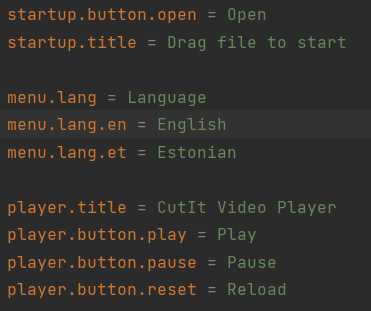
\includegraphics[width=0.6\textwidth]{Images/i18n.png}
    \caption{I18n faili sisu}
    \label{fig:i18n_example}
\end{figure}
Võti on igas keeles alati sama, kuid väärtus muutub sõltuvalt keelest. Lokaati tuleb määrata klassi Locale abil. FXML-failis tõlke kasutamiseks peate lihtsalt sisestama \% sümboli ja kirjutama vastava võtme (\nameref{fig:i18n_fxml}). 
\begin{figure}[H]
    \centering
    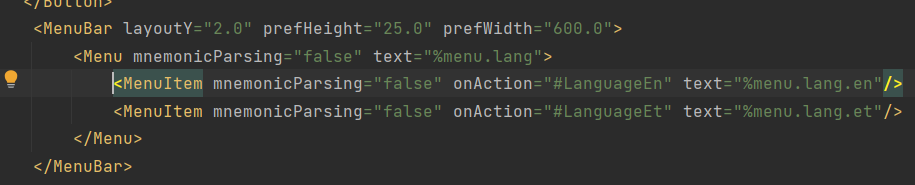
\includegraphics[width=1\textwidth]{Images/i18n_fxml.png}
    \caption{I18n kasutamine fxml failides}
    \label{fig:i18n_fxml}
\end{figure}
Rakenduse koodis tõlkimiseks on kaks võimalust: tõlkida terve aken, kasutades klassi fxmlLoader (\nameref{fig:i18n_code}) või muuta programmiliselt iga elemendi tekstiatribuuti. Projektis kasutatakse endist meetodit.
\begin{figure}[H]
    \centering
    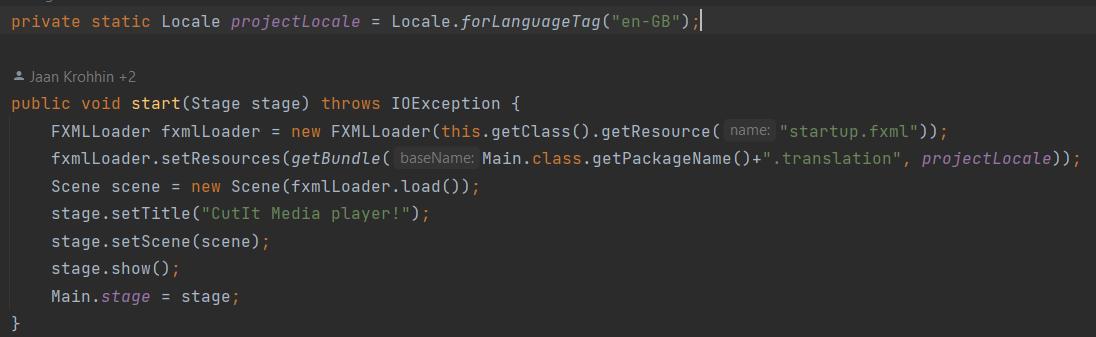
\includegraphics[width=1\textwidth]{Images/i18n_code.png}
    \caption{I18n kasutamine koodis}
    \label{fig:i18n_code}
\end{figure}

